\documentclass[11pt]{article}
\usepackage[utf8]{inputenc}
\usepackage[english]{babel}
\usepackage{multicol}
\setlength{\columnsep}{0.9525cm}
\usepackage{lipsum} 
\usepackage[a4paper,margin=1in,footskip=0.4in]{geometry}
\usepackage{times}
\usepackage{booktabs}
\usepackage{blindtext}
\bibliographystyle{unsrt}
\usepackage{todonotes}

\title{CCM Project}
\author{Luuk Arts (sxxxxxxx), Jordy Ripperda (s4381386), Jesse Zwamborn (sxxxxxxx)}
\date{June 2018}

\begin{document}
\twocolumn
[\maketitle
\begin{center}
    \section{Abstract}
\end{center}
*Insert abstract*
\vspace{0.5cm}
]


\section{Introduction}
Microblogging websites have enormously increased in popularity during the past years. One of the biggest examples is Twitter, which is an online news and social network site where users post and interact via tweets. Since Twitter is a real time platform, where users almost instantly tweet about varying types of events or topics, it can be a useful source of information for manufacturers or other persons of interest. For this reason Twitter mining, where tweets are used to for discovery, prediction or causality, has become very popular among companies and researchers. Examples of what has been done vary from simple sentiment analysis \cite{Agarwal2011, Go2009, Pak}, detecting epidemics \cite{Aramaki2011}, to predicting the stock market \cite{bollen2011twitter}. 

In this paper we will use tweets to predict the kind of weather, the sentiment corresponding to the weather, and whether the weather occurred in the present, past or future. The initial goal of our research was to also predict more specific temporal aspects, such as the season or the month of the year for example. However, since we could not find any applicable data for this, we decided to leave this out.

In order to do so the dataset of a Kaggle competition from five years ago will be used.\footnote{\url{https://www.kaggle.com/c/crowdflower-weather-twitter}} 
The competition was organized by CrowdFlower and the price money was \$500. CrowdFlower is a machine learning, training data, and artificial intelligence platform and has recently changed its name to Figure Eight. The dataset contains a set of tweets that are related to the weather that is labeled by humans, and the goal is to goal is to give predictions for three types of variables: sentiment, when and kind. There are five different sentiment labels and the goal is to predict each label with a certain probability. Each tweet can only correspond to one sentiment. The same rule applies to the 'when' labels. Each tweet can however have multiple 'kind' labels, which represent features such as windy or rainy. 

The winning strategy was relatively simple, as it used a ridge regression model with basic TF-IDF predictors of 1,2,3-grams and 3,5,6,7-grams as features. The outputs of the ridge regression model were then used as input for a second ensemble of forest models. This resulted in an root-mean-square error (RMSE) of 0.14313. 

The goal of this research is to reach the top 50 in the leaderbord, since the difference between the first and the 50th place is only 1\%. To do so we want to try different approaches.
\todo{zeg meer over onze approach}

\section{Methods}
\subsection{Data}
The first step in this project was an exploratory data analysis (EDA). Table \ref{rawdata} presents the first two instances from the raw training data and how it looks like exactly. The dataset contains 77946 tweets of training data and 42157 tweets of test data. 
\begin{table*}[t]
\begin{minipage}{\textwidth}
\centering
\resizebox{\textwidth}{!}{%
\begin{tabular}{@{}lrrrrrrrrrrrr@{}}
\toprule
\textbf{id} & \textbf{tweet}                       & \textbf{state} & \textbf{location}    & \textbf{s1} & \textbf{...} & \textbf{s5} & \textbf{w1} & \textbf{...} & \textbf{w4} & \textbf{k1} & \textbf{...} & \textbf{k15} \\ \midrule
1           & Jazz for a Rainy Afternoon: \{link\} & oklahoma       & Oklahoma             & 0.0         & ...          & 1.0         & 1.0         & ...          & 0.0         & 0.8         & ...          & 0.5          \\
2           & RT: @mention: I love rainy days.     & florida        & Miami-Ft. Lauderdale & 0.4         & ...          & 0.6         & 0.0         & ...          & 0.0         & 0.2         & ...          & 0.3          \\ \bottomrule
\end{tabular}}
\caption{Raw data}
\label{rawdata}
\end{minipage}
\end{table*}
Each tweet contains the tweet itself as a string, the state and location, five sentiment scores, four 'when' scores, and fifteen 'kind' scores.
As can be seen the sum of the sentiment and 'when' scores sum up to 1.0. This is because each tweet can only have one sentiment or 'when' score, however since multiple human annotators were used the probabilities are distributed. This does not hold for the 'kind' scores since each tweet can have multiple 'kind' labels (since they represent rainy or windy for example).

When looking at the distribution of the labels, we quickly came to the conclusion that data is quite unbalanced. Figure \ref{fig:dist} presents the distribution for the different categories. When looking at the kind of the weather, most tweets are assigned with the label "can't tell". When looking at the 'when' labels, you'll see that most tweets are about the current day. This seems reasonable since Twitter is a real-time platform. The sentiment labels are more equally distributed, but most tweets have a neutral sentiment.
\begin{figure*}[]
    \centering
    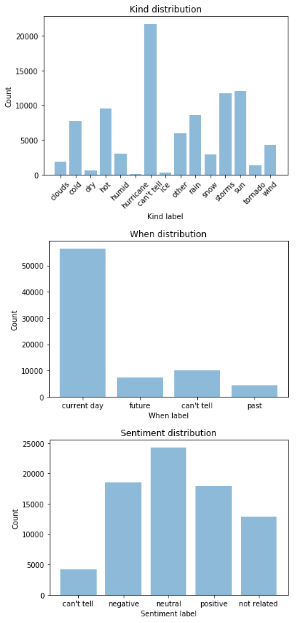
\includegraphics{distributions.png}
    \caption{The label distribution for the different categories}
    \label{fig:dist}
\end{figure*}

Finally, we searched whether there existed correlation between the different labels. We computed the correlations between each label, and used 0.3 as threshold. We also removed the correlations between two sentiment or 'when' labels, since each tweet can only have one of those. The correlation that remained were:
\begin{itemize}
    \item positive (sentiment) - sunny (kind): 0.37
    \item tweet not related to weather (sentiment) - current day (when): -0.38
    \item tweet not related to weather (sentiment) - can't tell (when): 0.45
    \item humid (kind) - wind (kind): 0.33
\end{itemize}


\subsection{Preprocessing}
The tweets are converted to lower case and stemming has been performed. Each tweet is tokenized using a tokenizer that is especially trained on and used for tweets. Stop words are removed from the tweets, together with words such as 'link', 'RT', 'facebook', 'twitter', 'google', etc. Finally elongated words (e.g. hotttt) are also removed.

\subsection{Features}

\subsection{Classifying}

\subsection{Post-processing}

\section{Results}

\section{Conclusion}




\newpage
\bibliography{references}


\end{document}
